\subsection{Validation of raw S2 GLAI observations against in-situ GLAI}

Figure \ref{fig:s2-obs-scatter-plots} shows the raw \gls{S2} \gls{GLAI} observations plotted against in-situ measured \gls{GLAI} with a maximum temporal offset of one day. The \gls{RMSE} was about 1.16 $m^2$ $m^{-2}$ (\gls{nRMSE} 18.92\%) with a bias of 1.87 $m^2$ $m^{-2}$. The raw \gls{S2} \gls{GLAI} observations explained 64\% of the variability in the in-situ values. The raw \gls{S2} \gls{GLAI} values showed a clear underestimation of in-situ \gls{GLAI} > 5 $m^2$ $m^{-2}$ in 2022 (blue dots in Figure \ref{fig:s2-obs-scatter-plots}) as well as three isolated outliers in 2023 (cross markers) for in-situ \gls{GLAI} values between 2 and 3 $m^2$ $m^{-2}$. Due to high cloud cover, only 8 out of 55 available observations for validation were recorded in 2023. Therefore, no year effects could be studied. The same applies to the phenological macro-stages for which not enough data was available to compute robust error statistics.

\begin{figure}[H]
    \centering
    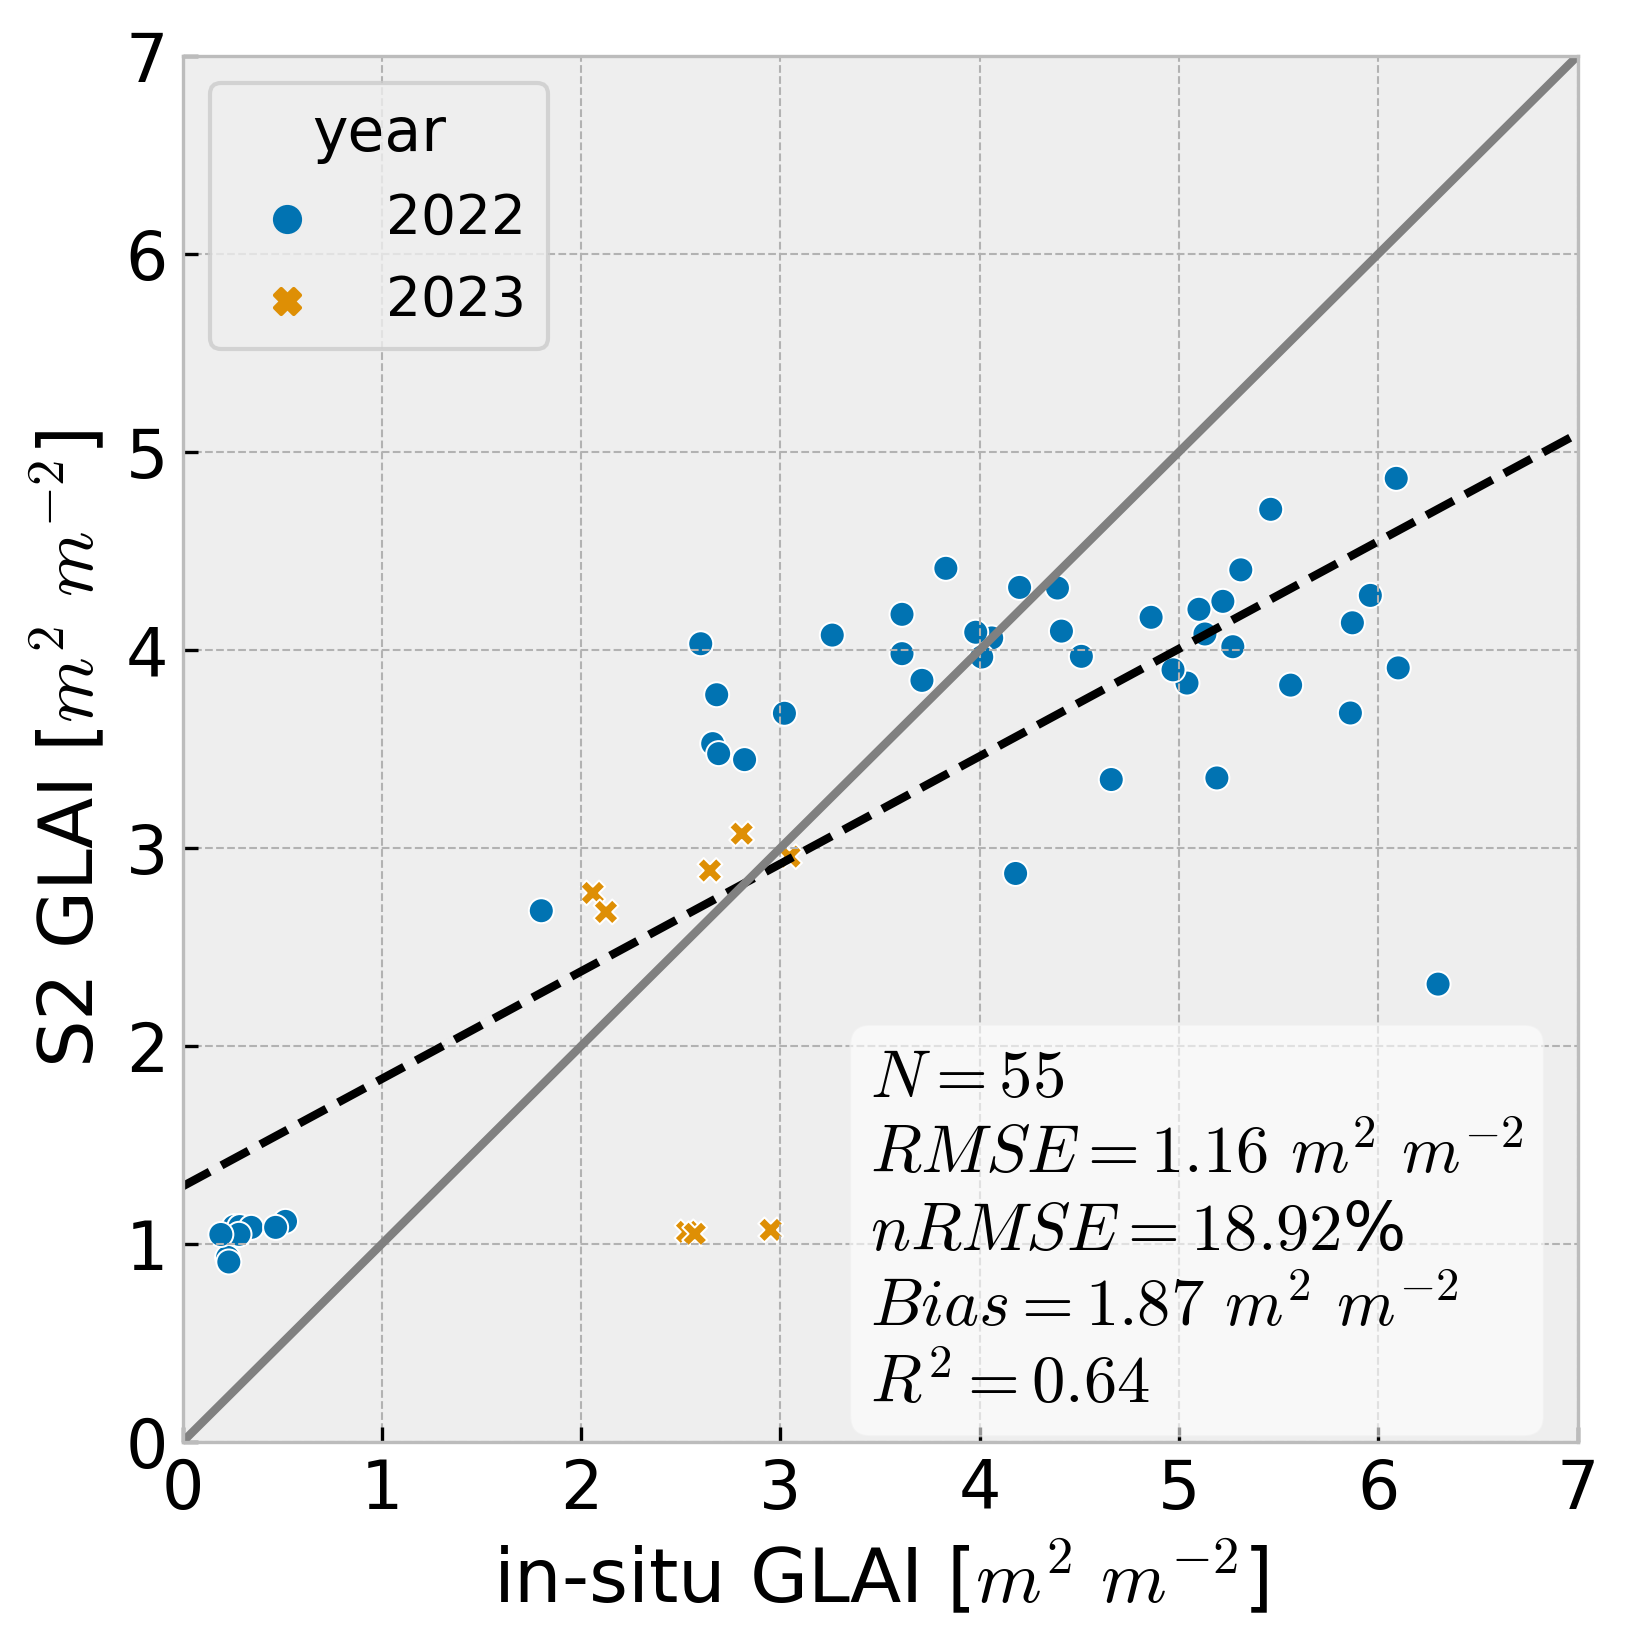
\includegraphics{s2_glai-obs_validation.png}
    \caption{Scatter plots of S2 observed and in-situ measured GLAI at the validation sites using data from 2022 and 2023. The oblique solid lines denotes the desired 1:1 fit; the dashed line denotes the linear regression line between S2 observed and in-situ measured \gls{GLAI} values. N = 55. The years are color-coded.}
    \label{fig:s2-obs-scatter-plots}
\end{figure}

\subsection{Validation of reconstructed GLAI time series against in-situ GLAI}
Similar to Figure \ref{fig:s2-obs-scatter-plots}, scatter plots of reconstructed GLAI (i.e., \gls{DRC} and baseline \gls{GLAI}) at hourly and daily resolution against in-situ measured \gls{GLAI} are displayed in Figure~\ref{fig:glai-scatter-plots} (N = 178). Figure~\ref{fig:glai-scatter-plots} (a-c) shows the results of the proposed \gls{DRC} GLAI time series, and (d) the baseline \gls{GLAI} results which are available in daily resolution, only. The error statistics are listed in Table~\ref{tab:error-stats}.

All models revealed a tendency to overestimate low in-situ \gls{GLAI} (< 1.0 $m^2$ $m^{-2}$). The baseline (Figure~\ref{fig:glai-scatter-plots}d) clearly underestimated in-situ \gls{GLAI} values > 5.0 $m^2$ $m^{-2}$. All models performed similar in terms of \gls{RMSE}, \gls{nRMSE} and \gls{R2} (Table~\ref{tab:error-stats}). The hourly asymptotic \gls{DRC} \gls{GLAI} had the smallest \gls{RMSE} (0.98 $m^2$ $m^{-2}$) closely followed by the daily asymptotic and non linear \gls{DRC} \gls{GLAI} (\gls{RMSE} around 0.99  $m^2$ $m^{-2}$, \gls{nRMSE} around 15\%). The highest \gls{RMSE} was observed for the Wang Engels \gls{DRC} \gls{GLAI} at hourly resolution (1.12  $m^2$ $m^{-2}$, \gls{nRMSE}: 17.43\%). The baseline \gls{GLAI} had a slightly lower \gls{RMSE} (1.05  $m^2$ $m^{-2}$, \gls{nRMSE}: 16.27\%) than the daily Wang Engels \gls{DRC} \gls{GLAI} (1.06  $m^2$ $m^{-2}$). A similar picture revealed \gls{R2} which ranged between 0.54 (Wang Engels hourly \gls{DRC} \gls{GLAI}) and 0.70 (non linear daily \gls{DRC} \gls{GLAI}). The highest bias was observed for the baseline \gls{GLAI} (1.66  $m^2$ $m^{-2}$). This was higher than for the \gls{DRC} \gls{GLAI} and more than two times larger than the smallest bias (0.73  $m^2$ $m^{-2}$) obtained from the hourly Wang Engels \gls{DRC} \gls{GLAI} which had the lowest bias.

\begin{figure}[H]
    \centering
    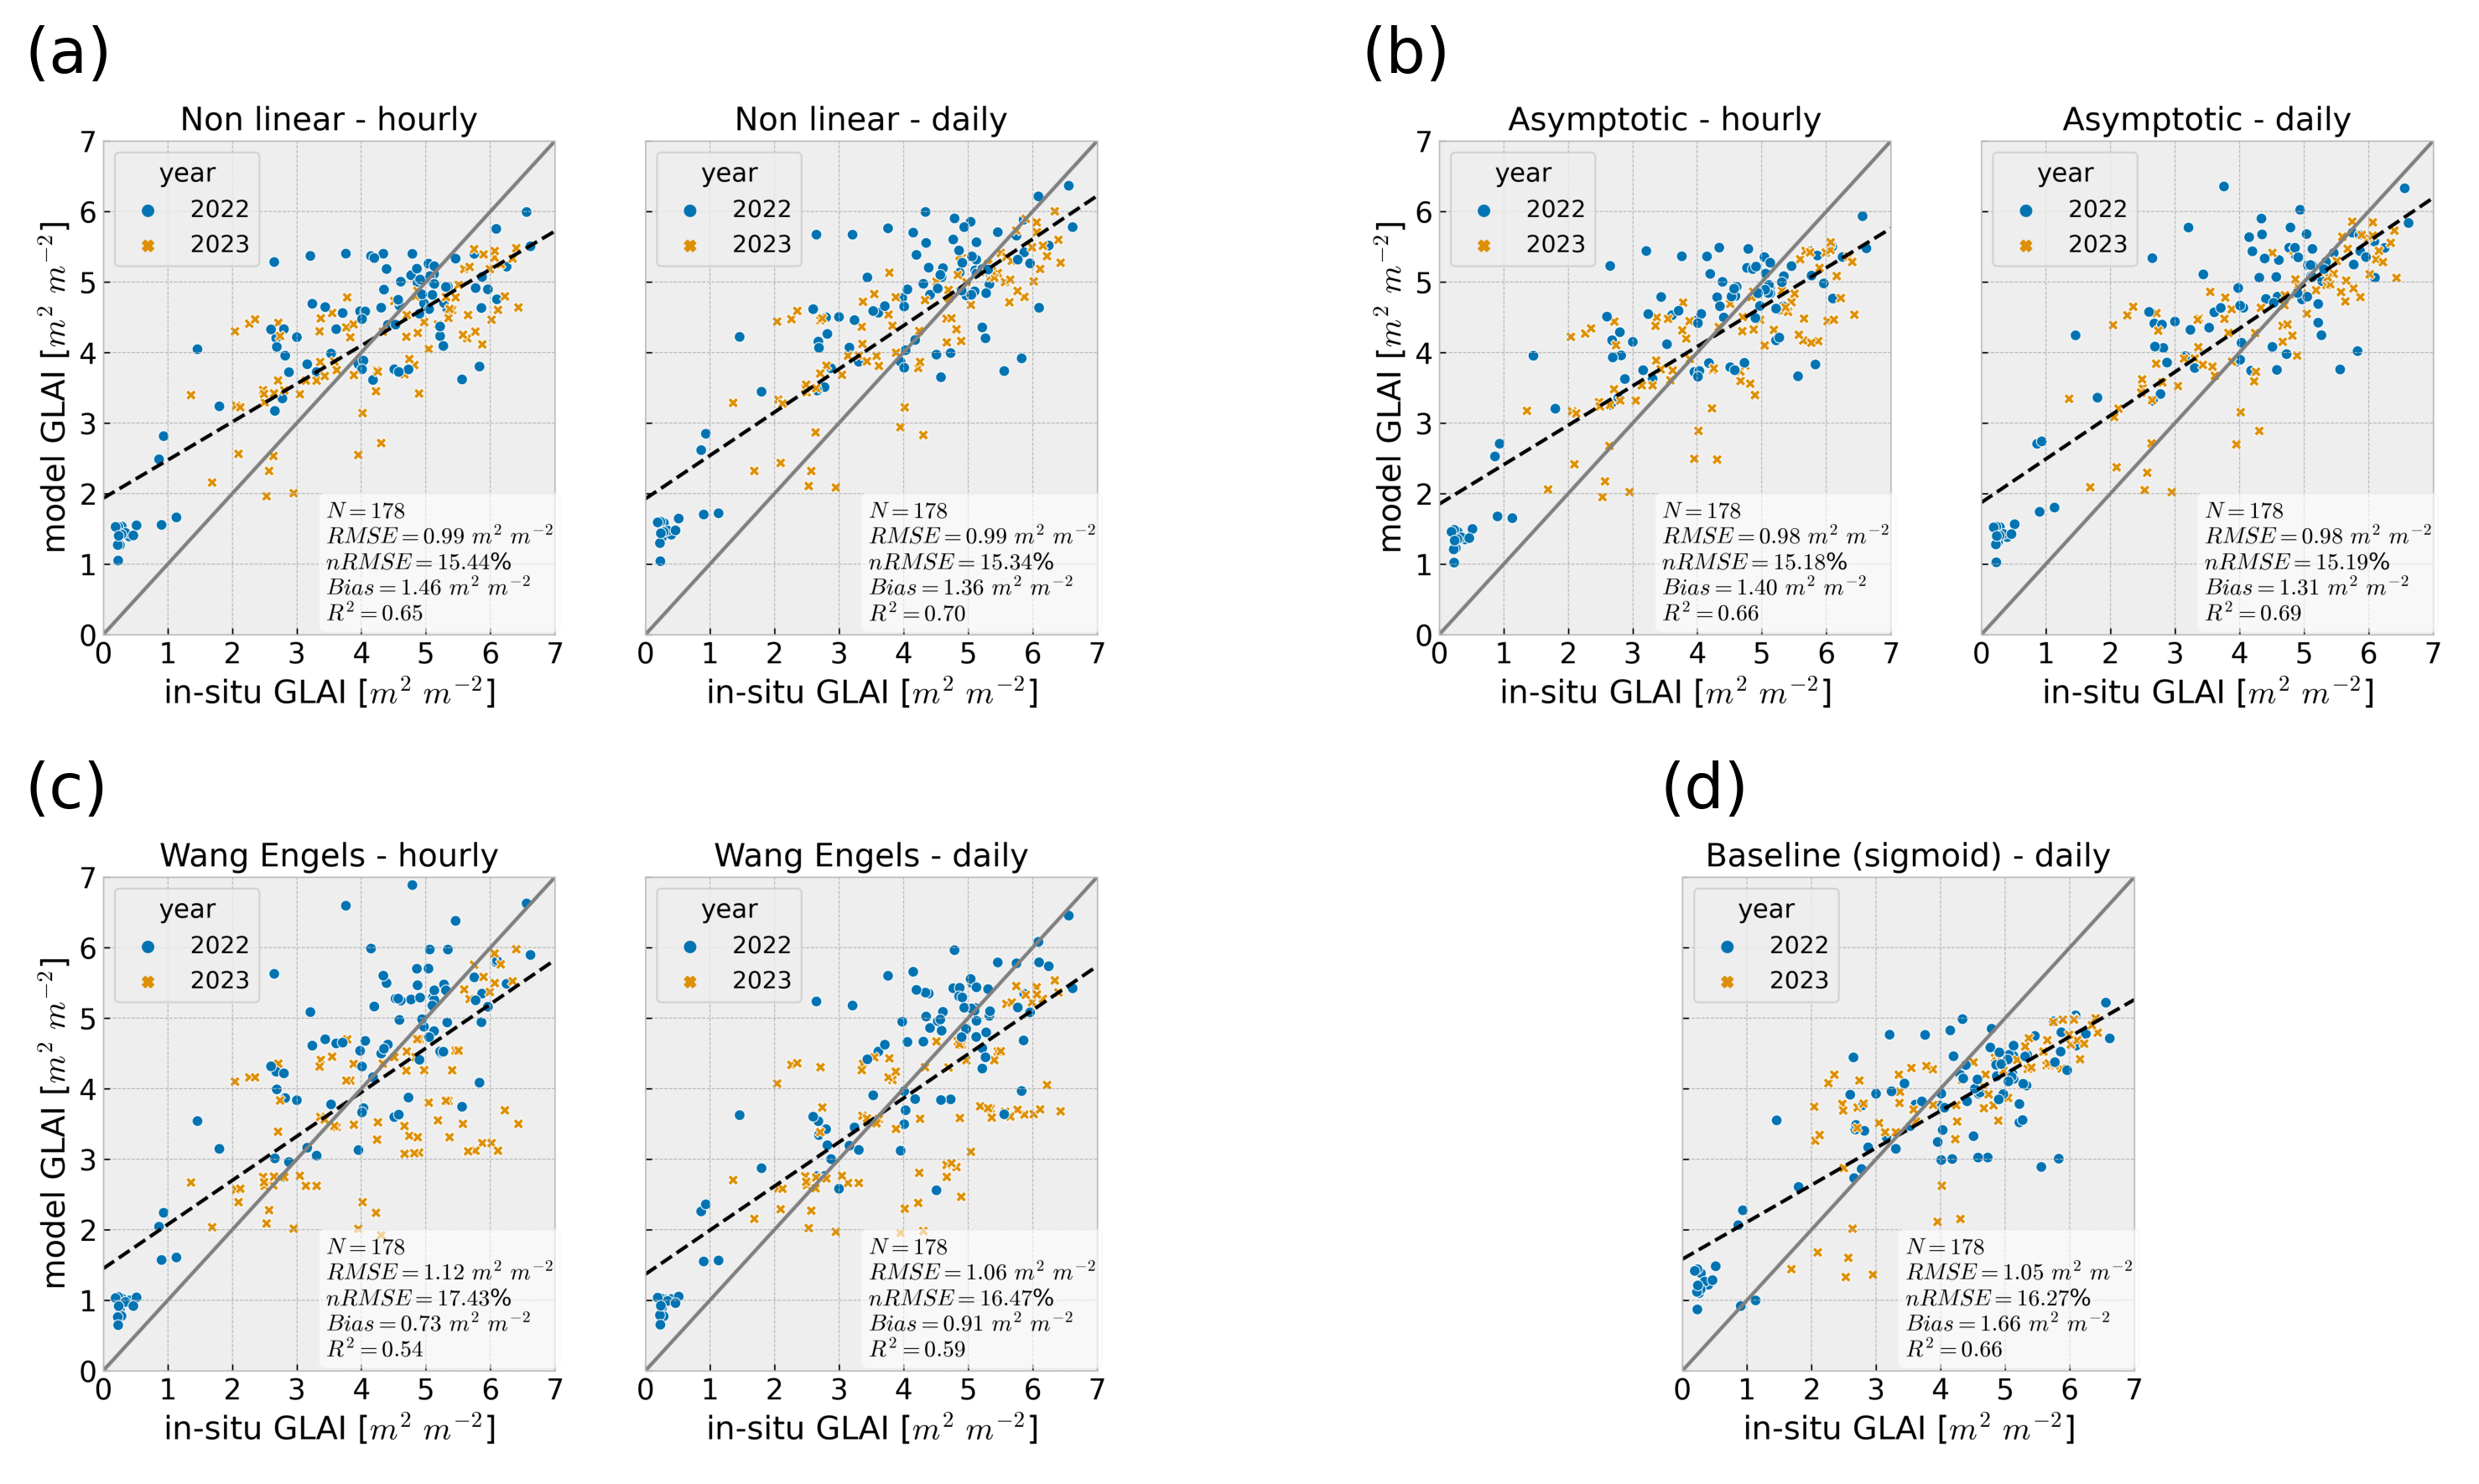
\includegraphics[width=\textwidth]{glai_scatter_plots.png}
    \caption{Scatter plots between reconstructed \gls{DRC} (a-c) and baseline (d) \gls{GLAI} and in-situ \gls{GLAI} at the validation sites using data from 2022 and 2023 (color-coded). For each \gls{DRC} \gls{GLAI}, the results using hourly and daily mean air temperature are shown (a-c). The baseline \gls{GLAI} is only available in daily resolution (d). The oblique solid line denotes the desired 1:1 fit and the dashed line the linear regression line between reconstructed and in-situ \gls{GLAI} values. N = 178.}
    \label{fig:glai-scatter-plots}
\end{figure}

\begin{table}[H]
\caption{Error statistics of reconstructed and in-situ \gls{GLAI} values (N = 178). \gls{RMSE} and bias are given in $m^2$ $m^{-2}$, \gls{nRMSE} in percent and \gls{R2} is dimensionless.}
\label{tab:error-stats}
\centering
\begin{tabular}{@{}llllll@{}}
\toprule
model                        & resolution & \gls{RMSE}          & \gls{nRMSE}         & Bias          & \gls{R2}            \\ \midrule
\multirow{2}{*}{Non linear} & hourly      & 0.99          &  15.44 & 1.46          & 0.65          \\
                             & daily       & 0.99          & 15.34 & 1.36          & 0.70 \\
\multirow{2}{*}{Asymptotic}  & hourly      & 0.98 & 15.17 & 1.40          & 0.66          \\
                             & daily       & 0.98 & 15.19 & 1.31          & 0.69          \\
\multirow{2}{*}{Wang Engels}  & hourly      & 1.12          & 17.43          & 0.73 & 0.54          \\
                             & daily       & 1.06          & 16.47          & 0.91          & 0.59          \\
Baseline (sigmoid)                      & daily       & 1.05          & 16.27          & 1.66          & 0.66          \\ \bottomrule
\end{tabular}
\end{table}

\subsubsection{Effect of the years}
Error statistics by year are shown in Table~\ref{tab:error-stats-years}. Arrows in table indicate whether a metric value remain unchanged ($\rightarrow$), decrease ($\downarrow$), or increased ($\uparrow$) from 2022 to 2023. For all models and temporal resolutions, the relative error was higher and $R^2$ lower in 2023 (N = 82) than 2022 (N = 96). In 2022, nRMSE values ranged from 13.04 (Wang Engels daily) to 16.72\% (non linear daily), while $R^2$ took values between 0.74 (baseline) and 0.8 (Wang Engels daily). In 2023, nRMSE values were in the range between 17.16 (asymptotic daily) and 25.62\% (Wang Engels hourly) with $R^2$ between 0.3 (Wang Engels hourly) and 0.62 (non linear daily). The RMSE was higher in 2023 than 2022 in four cases (asymptotic hourly, Wang Engels hourly and daily, and the baseline), unchanged in one case (non linear hourly), and decreased in the remaining two cases (non linear daily and asymptotic daily). The highest RMSE was obtained from the hourly Wang Engels \gls{DRC} in 2023 (1.30 $m^2$ $m^{-2}$, value in 2022: 0.94 $m^2$ $m^{-2}$), the lowest for the Wang Engels \gls{DRC} in 2022 (0.84 $m^2$ $m^{-2}$, value in 2023: 1.27 $m^2$ $m^{-2}$). The bias decreased in all cases in 2023 compared to 2022 except the Wang Engels \gls{DRC}: Here, the bias increased from 0.83 to 1.10 $m^2$ $m^{-2}$ (hourly) and from 0.90 to 1.22 $m^2$ $m^{-2}$ (daily).

%In 2022 (N = 96), \gls{DRC} and baseline \gls{GLAI} accuracy was mostly higher than in 2023 (N = 82). In 2022, \gls{R2} ranged from 0.74 for the baseline to 0.8 for the daily Wang Engels \gls{DRC} \gls{GLAI} (Table~\ref{tab:error-stats-2022}). In 2023, \gls{R2} values were lower ranging between 0.3 (Wang Engels hourly \gls{DRC} \gls{GLAI}) and 0.62 (non linear daily \gls{DRC} \gls{GLAI}). The bias was mostly higher in 2022 ranging between 0.83 $m^2$ $m^{-2}$ for the Wang Engels hourly \gls{DRC} \gls{GLAI} to 1.96 $m^2$ $m^{-2}$ for the baseline \gls{GLAI}. In 2023, the bias was highest for the daily Wang Engels \gls{DRC} \gls{GLAI} (1.22 $m^2$ $m^{-2}$) and lowest for the daily asymptotic \gls{DRC} \gls{GLAI} (0.96 $m^2$ $m^{-2}$).

%Overall, the Wang Engels \gls{DRC} \gls{GLAI} showed the most pronounced differences between the years. In 2022, the \gls{RMSE} of the Wang Engels \gls{DRC} \gls{GLAI} was about 0.94 and 0.84 $m^2$ $m^{-2}$ for the hourly and daily model, respectively (\gls{nRMSE} around 15 and 13\%). In 2023 (N = 82), the \gls{RMSE} decreased to 1.30 and 1.27 $m^2$ $m^{-2}$ (nRMSE: 24 and 25\%, respectively).

%\begin{table}[H]
%\caption{Error statistics of reconstructed and in-situ \gls{GLAI} values in 2022 (N = 96). \gls{RMSE} and bias are given in $m^2$ $m^{-2}$, \gls{nRMSE} in percent and \gls{R2} is dimensionless.}
%\label{tab:error-stats-2022}
%\centering
%\begin{tabular}{@{}llllll@{}}
%\toprule
%model                        & resolution & \gls{RMSE} & \gls{nRMSE} & Bias & \gls{R2}   \\ \midrule
%\multirow{2}{*}{Non linear} & hourly     & 0.99 & 15.44 & 1.71 & 0.75 \\
%                             & daily      & 1.07 & 16.72 & 1.64 & 0.75 \\
%\multirow{2}{*}{Asymptotic}  & hourly     & 0.96 & 14.98 & 1.66 & 0.77 \\
%                             & daily      & 1.06 & 16.47 & 1.60 & 0.75 \\
%\multirow{2}{*}{Wang Engels}  & hourly     & 0.94 & 14.64 & 0.83 & 0.77 \\
%                             & daily      & 0.84 & 13.04 & 0.90 & 0.80 \\ 
%Baseline (sigmoid)           & daily      & 1.03 & 15.97 & 1.96 & 0.74 \\ \bottomrule
%\end{tabular}
%\end{table}

\begin{table}[H]
    \centering
    \caption{Error statistics of reconstructed and in-situ \gls{GLAI} values in 2022 (N = 96) and 2023 (N = 82). The arrows indicate the change in the metrics from 2022 to 2023: $\uparrow$ means the value increased in 2023 compared to 2022, $\downarrow$ it decreased, and $\rightarrow$ it remained unchanged. \gls{RMSE} and bias are given in $m^2$ $m^{-2}$, \gls{nRMSE} in percent and \gls{R2} is dimensionless.}
    \label{tab:error-stats-years}
\begin{tabular}{@{}llllllllllllll@{}}
\toprule
model                        & resolution & \multicolumn{3}{l}{RMSE} & \multicolumn{3}{l}{nRMSE} & \multicolumn{3}{l}{Bias} & \multicolumn{3}{l}{$R^2$} \\ \midrule
                             &            & 2022    & 2023     &             & 2022     & 2023     &            & 2022   & 2023   &             & 2022   & 2023   &     \\ \cmidrule(l){2-14} 
\multirow{2}{*}{Non linear}  & hourly     & 0.99  & 0.99  & $\rightarrow$ & 15.44  & 19.58  & $\uparrow$  & 1.71 & 1.18 & $\downarrow$ & 0.75 & 0.49 & $\downarrow$ \\
                             & daily      & 1.07  & 0.87  & $\downarrow$  & 16.72  & 17.18  & $\uparrow$  & 1.64 & 1.01 & $\downarrow$ & 0.75 & 0.62 & $\downarrow$ \\ \cmidrule(l){2-14} 
\multirow{2}{*}{Asymptotic}  & hourly     & 0.96  & 0.99  & $\uparrow$    & 14.98  & 19.52  & $\uparrow$  & 1.66 & 1.14 & $\downarrow$ & 0.77 & 0.50 & $\downarrow$  \\
                             & daily      & 1.06  & 0.87  & $\downarrow$  & 16.47  & 17.16  & $\uparrow$  & 1.60 & 0.96 & $\downarrow$ & 0.75 & 0.60 & $\downarrow$  \\ \cmidrule(l){2-14} 
\multirow{2}{*}{Wang Engels} & hourly     & 0.94  & 1.30  & $\uparrow$    & 14.64  & 25.62  & $\uparrow$  & 0.83 & 1.10 & $\uparrow$   & 0.77 & 0.30 & $\downarrow$  \\
                             & daily      & 0.84  & 1.27  & $\uparrow$    & 13.04  & 25.02  & $\uparrow$  & 0.90 & 1.22 & $\uparrow$   & 0.80 & 0.33 & $\downarrow$  \\ \cmidrule(l){2-14} 
\shortstack{Baseline\\(sigmoid)} & daily      & 1.03  & 1.07  & $\uparrow$    & 15.97  & 22.55  & $\uparrow$  & 1.96 & 1.21 & $\downarrow$ & 0.74 & 0.48 & $\downarrow$  \\ \bottomrule
\end{tabular}
\end{table}


%\begin{table}[H]
%\caption{Error statistics of reconstructed and in-situ \gls{GLAI} values in 2023 (N = 82). \gls{RMSE} and bias are given in $m^2$ $m^{-2}$, \gls{nRMSE} in percent and \gls{R2} is dimensionless.}
%\label{tab:error-stats-2023}
%\centering
%\begin{tabular}{@{}llllll@{}}
%\toprule
%model                        & resolution & \gls{RMSE} & \gls{nRMSE} & Bias & \gls{R2}   \\ \midrule
%\multirow{2}{*}{Non linear}  & hourly     & 0.99 & 19.58 & 1.18 & 0.49 \\
%                             & daily      & 0.87 & 17.18 & 1.01 & 0.62 \\
%\multirow{2}{*}{Asymptotic}  & hourly     & 0.99 & 19.52 & 1.14 & 0.50 \\
%                            & daily      & 0.87 & 17.16 & 0.96 & 0.60 \\
%\multirow{2}{*}{Wang Engels} & hourly     & 1.30 & 25.62 & 1.10 & 0.30 \\
%                             & daily      & 1.27 & 25.02 & 1.22 & 0.33 \\
%Baseline (sigmoid)           & daily      & 1.07 & 22.55 & 1.21 & 0.48 \\ \bottomrule
%\end{tabular}
%\end{table}

\subsubsection{Effect of phenology}
The \gls{GLAI} reconstruction errors were dependent on the phenological macro-stage. Figure~\ref{fig:glai-errors-phenology} shows the error measures for \gls{BBCH} macro stages 30-39 (stem elongation), and 50-59 (heading) for the \gls{DRC} and baseline with daily \gls{GLAI} output. There were too few in-situ data for the booting stage (N = 5) available, so we restricted our analysis to stem elongation (N = 136) and heading (N = 37). For these stages, the baseline \gls{GLAI} exhibited the largest bias (1.6 and 1.2 $m^2$ $m^{-2}$, respectively). During heading, the baseline \gls{GLAI} also showed largest \gls{RMSE} (around 1.2 $m^2$ $m^{-2}$) and its bias was almost twice as high as in the \gls{DRC} \gls{GLAI} (bias around 0.6 $m^2$ $m^{-2}$). The difference in \gls{R2} was less pronounced; the \gls{DRC} and baseline \gls{GLAI} had a high \gls{R2} in stem elongation (0.55 to 0.73), which decreased significantly during heading (0.05 to 0.15). Overall, the differences between the three \gls{DRC} \gls{GLAI} models were less pronounced than the difference between these models and the baseline \gls{GLAI}.

\begin{figure}[H]
    \centering
    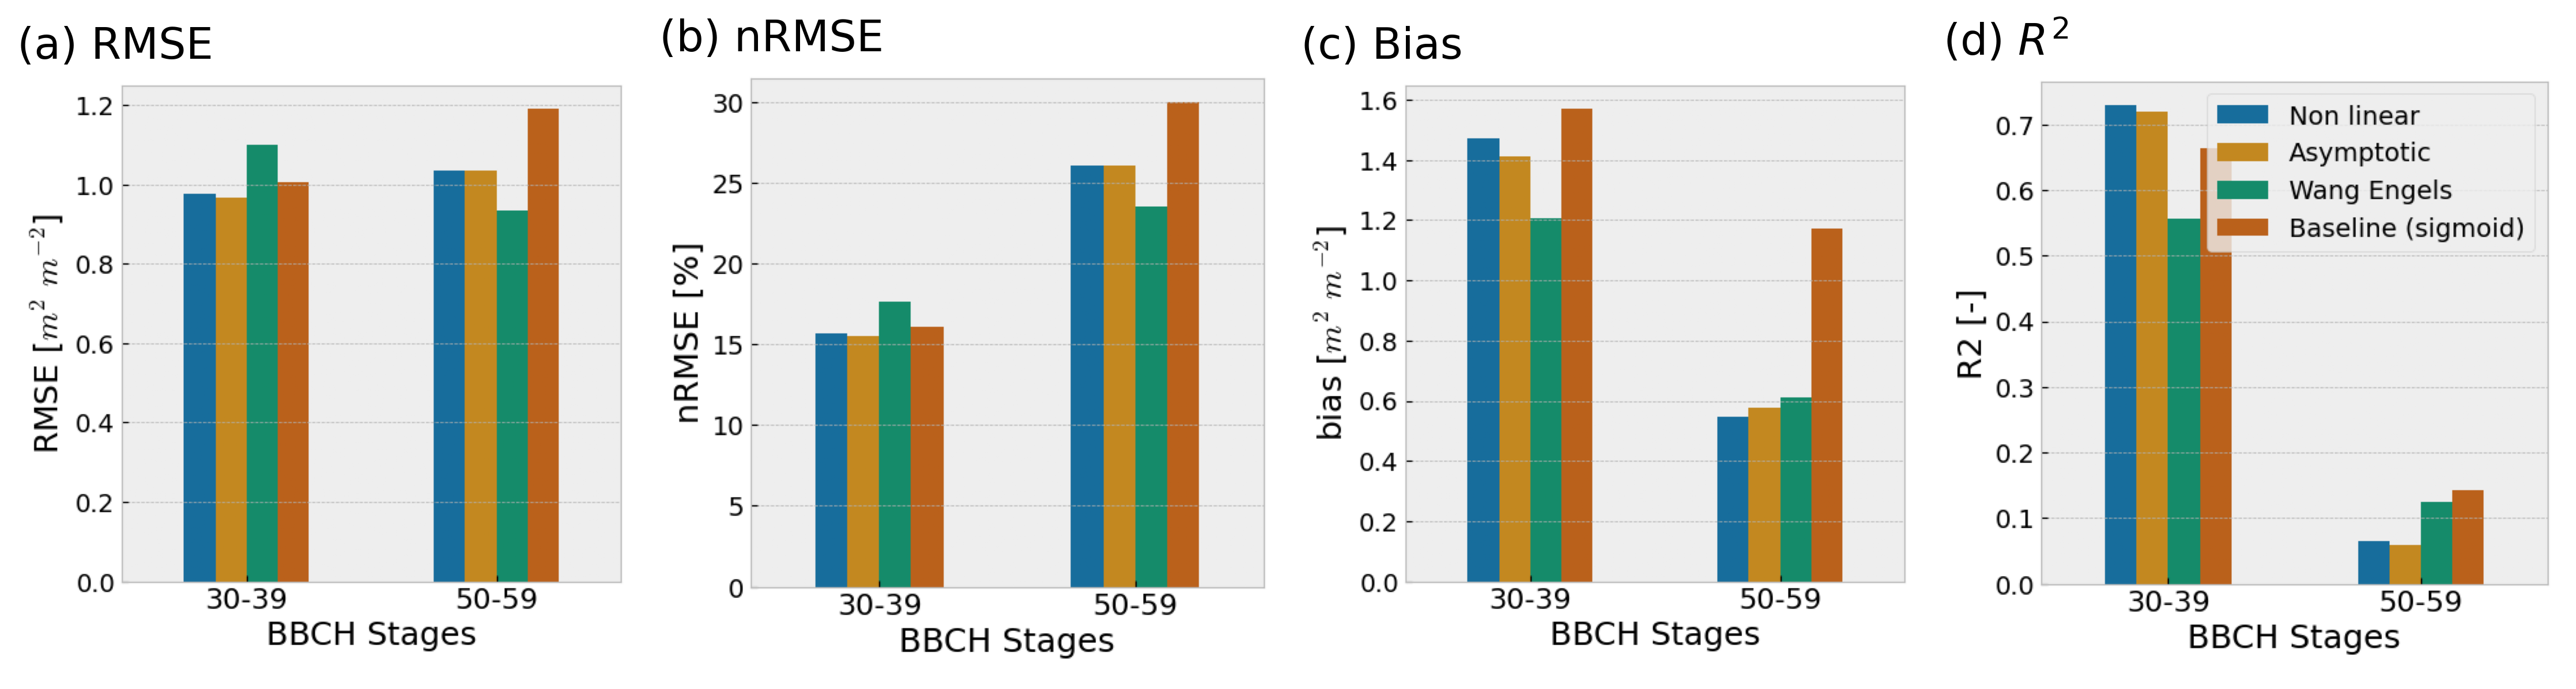
\includegraphics[width=\textwidth]{glai_daily-error_plots-bbch.png}
    \caption{Reconstructed versus in-situ \gls{GLAI} error statistics per BBCH macro-stage and model. Only the results of the daily \gls{DRC} \gls{GLAI} are shown.}
    \label{fig:glai-errors-phenology}
\end{figure}

\subsubsection{Time series reconstruction}

Figure~\ref{fig:glai-trajectories} visualizes the reconstructed median \gls{DRC} and baseline \gls{GLAI} time series at daily resolution in \gls{DAS} per field parcel and year (see also Figure~\ref{fig:map-validation-sites}). The spatial in-field variability obtained from each model is shown as filled areas color-coded by model. The in-situ \gls{GLAI} values are plotted as blue dots to allow comparison of reconstructed versus measured in-field heterogeneity and temporal dynamics. Both, \gls{DRC} and baseline \gls{GLAI} show an increase in \gls{GLAI} from the beginning of the stem elongation to the end heading, which largely reflects the dynamics of the in situ data.

The asymptotic (dotted green) and non linear (solid golden) \gls{DRC} \gls{GLAI} were able to accurately reconstruct in-situ \gls{GLAI} spatial variability and reflect the temporal trajectories of the in-situ \gls{GLAI} values. These models were able to represent the higher in-situ \gls{GLAI} (> 5 $m^2$ $m^{-2}$) during late booting and heading. Wang Engels \gls{DRC} \gls{GLAI} (dash-dotted brown) mostly followed similar trajectories but with a tendency towards a delayed increase in \gls{GLAI} evident in the 2023 plots (Figure~\ref{fig:glai-trajectories}e-g). In addition, the Wang Engels \gls{DRC} \gls{GLAI} showed a less smooth progression than the other two \gls{DRC} \gls{GLAI} models and the baseline, as evidenced by jumps and plateaus in the median GLAI time series (Figure~\ref{fig:glai-trajectories}).

The baseline \gls{GLAI} (dashed blue) showed the expected smooth progression. While in-situ \gls{GLAI} at the beginning and middle of the time series are still reproduced largely accurately, the underestimation of higher in-situ \gls{GLAI} values (>5 $m^2$ $m^{-2}$) is clearly evident in Figure~\ref{fig:glai-trajectories}. In Figure~\ref{fig:glai-trajectories}g, the baseline \gls{GLAI} also revealed a rapid increase in GLAI between \gls{DAS} 160 and 180 from 0.5 to 3.5 $m^2$ $m^{-2}$ which is not present in the \gls{DRC} \gls{GLAI} time series.

\begin{figure}[H]
    \centering
    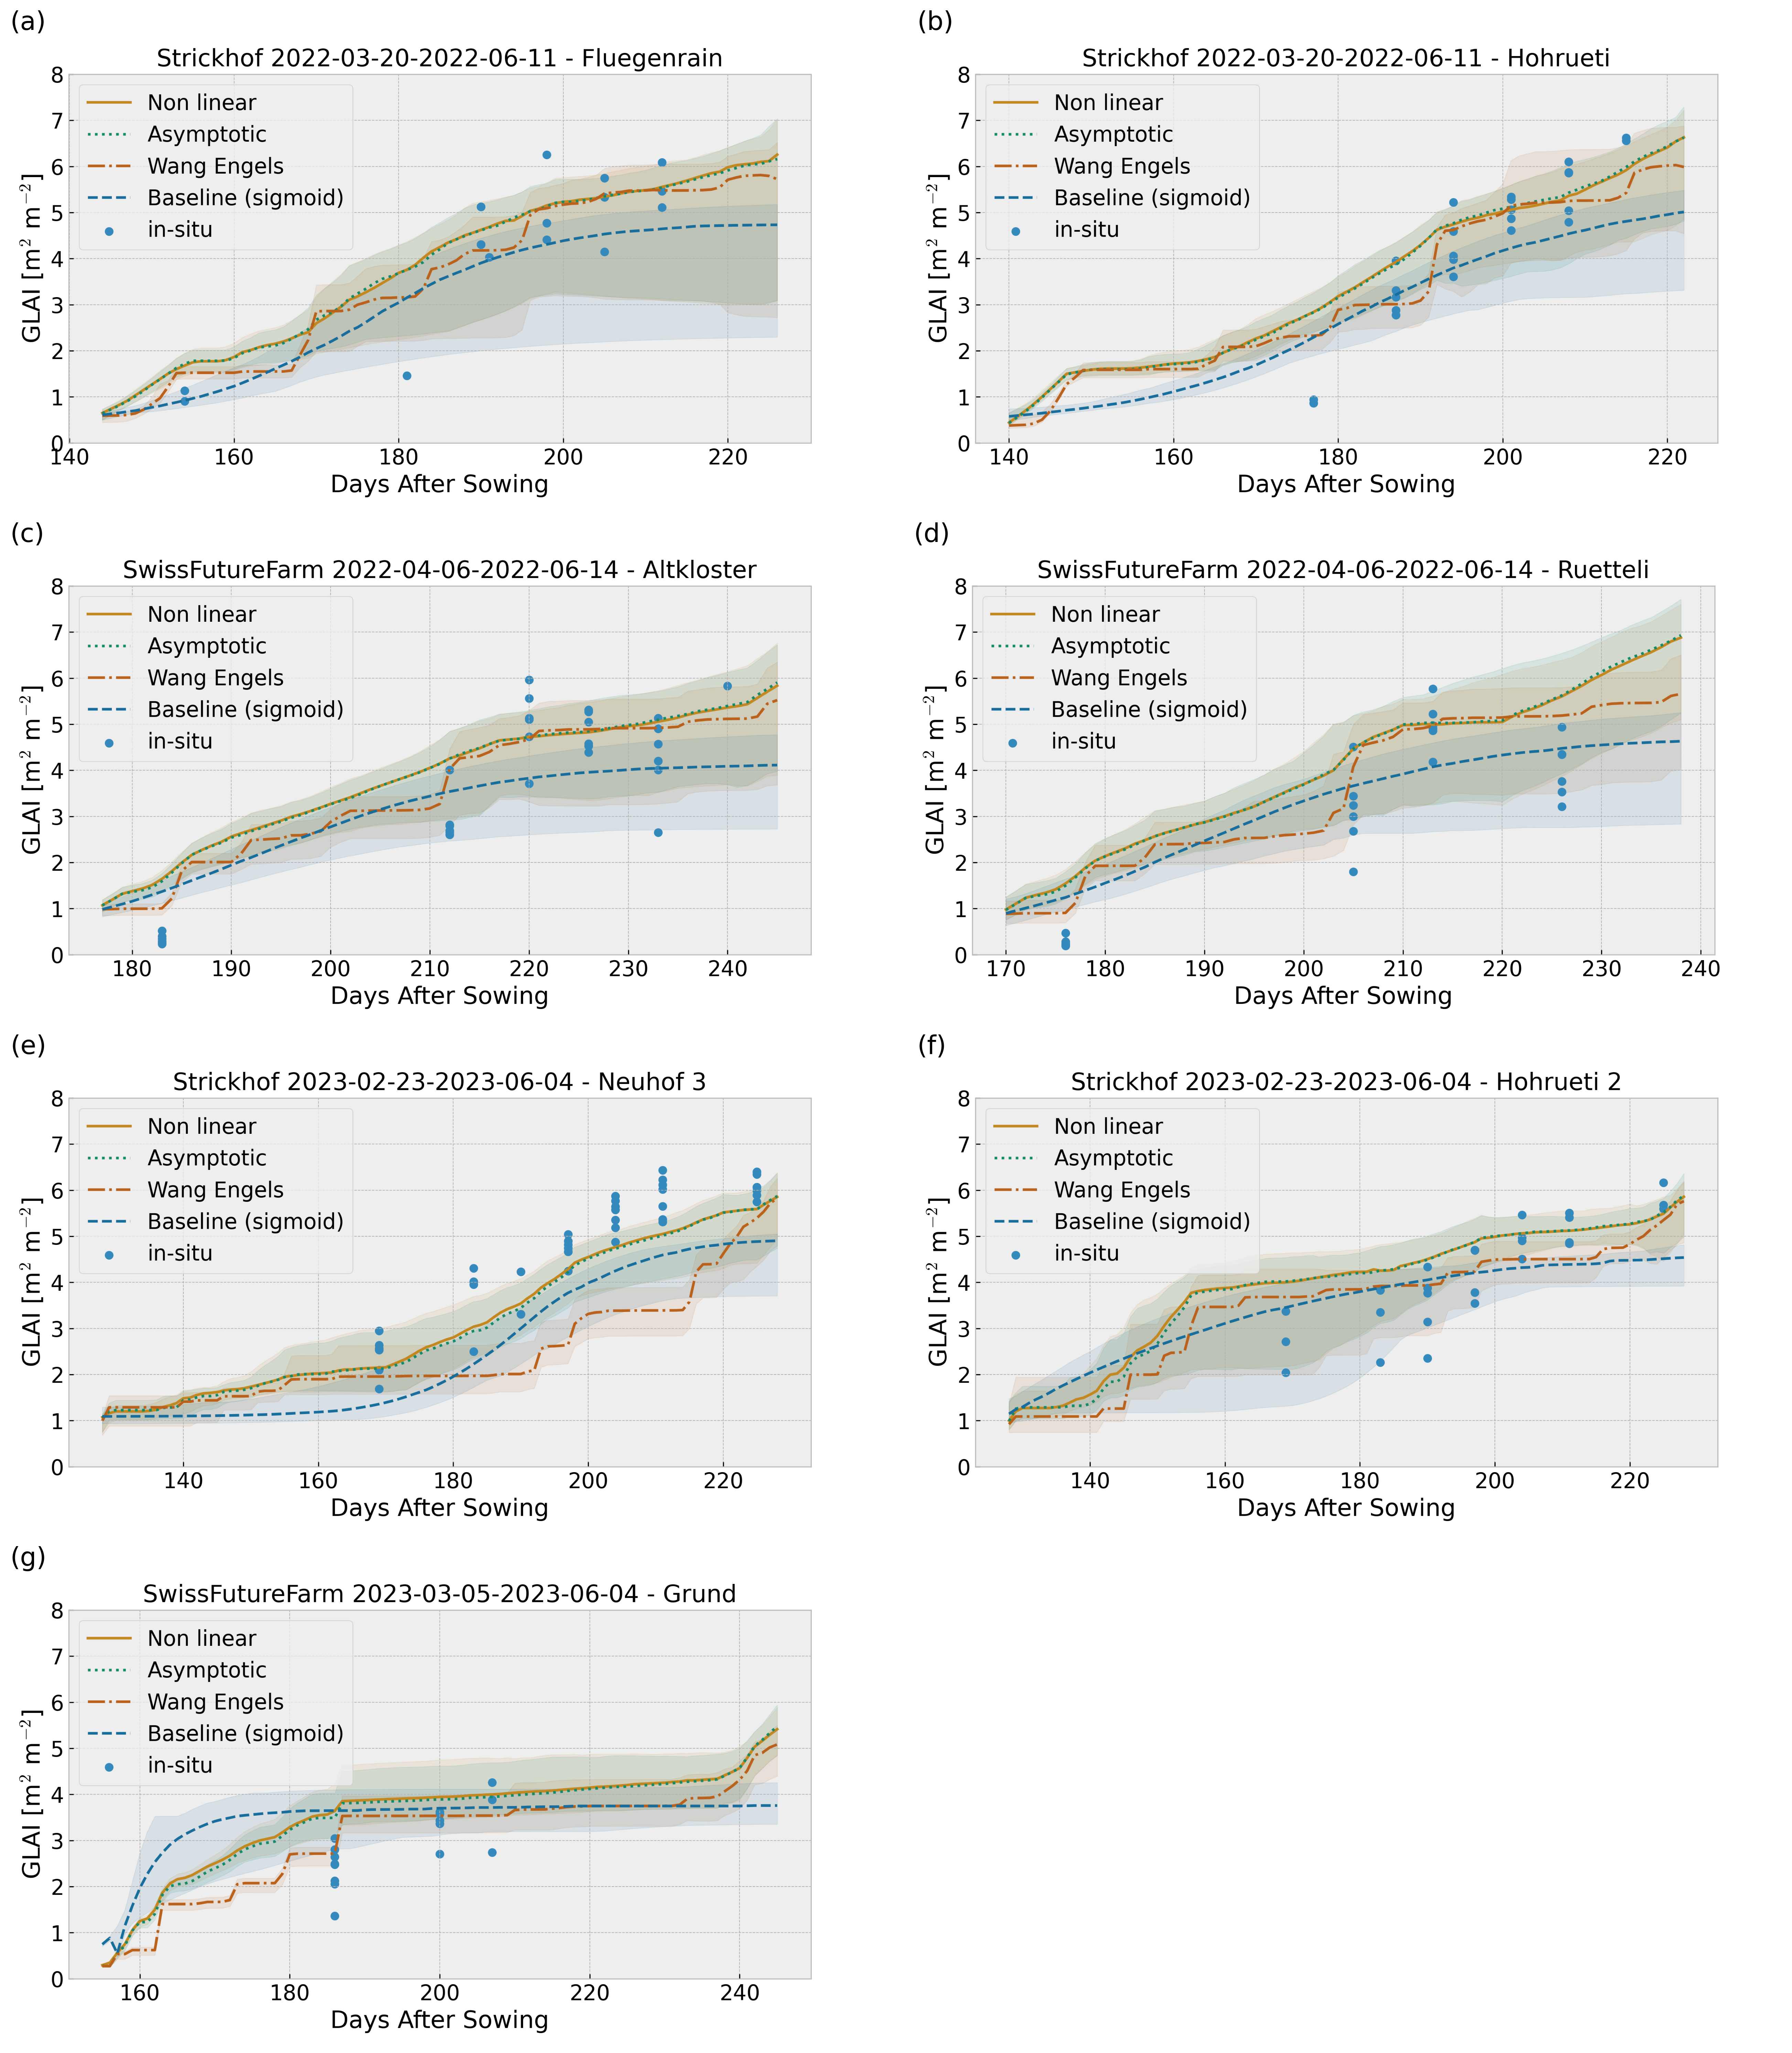
\includegraphics[width=\textwidth]{glai_daily-temporal_profiles.png}
    \caption{Median daily reconstructed \gls{DRC} and baseline \gls{GLAI} time series (lines) and spatial in-field variability in terms of the 5\% to 95\% percentile spread (filled areas) at the field parcels of the validation site (Figure~\ref{fig:map-validation-sites}). The in-situ \gls{GLAI} values are denoted as blue dots.}
    \label{fig:glai-trajectories}
\end{figure}

To further highlight the difference between the \gls{DRC} and the baseline \gls{GLAI}, we plotted the daily asymptotic \gls{DRC} \gls{GLAI} which achieved overall high accuracy (see Tables \ref{tab:error-stats}-\ref{tab:error-stats-years}), against the baseline \gls{GLAI} considering all pixels and dates. The resulting scatter plots are shown for each validation site and year in Figure \ref{fig:model-intercomparison}. In Figure \ref{fig:model-intercomparison}a-c it becomes clear that the baseline \gls{GLAI} reconstructed slightly lower \gls{GLAI} values than the asymptotic \gls{DRC}. The effect was particularly pronounced for GLAI values > 5 $m^2$ $m^{-2}$, as shown by the systematic deviation from the 1:1 line. In Figure \ref{fig:model-intercomparison}d the effect is less pronounced. This site (Swiss Future Farm 2023), however, was also affected by a high proportion of pixels that could not be reconstructed in the baseline \gls{GLAI}, as we will show in the next section.

\begin{figure}[H]
    \centering
    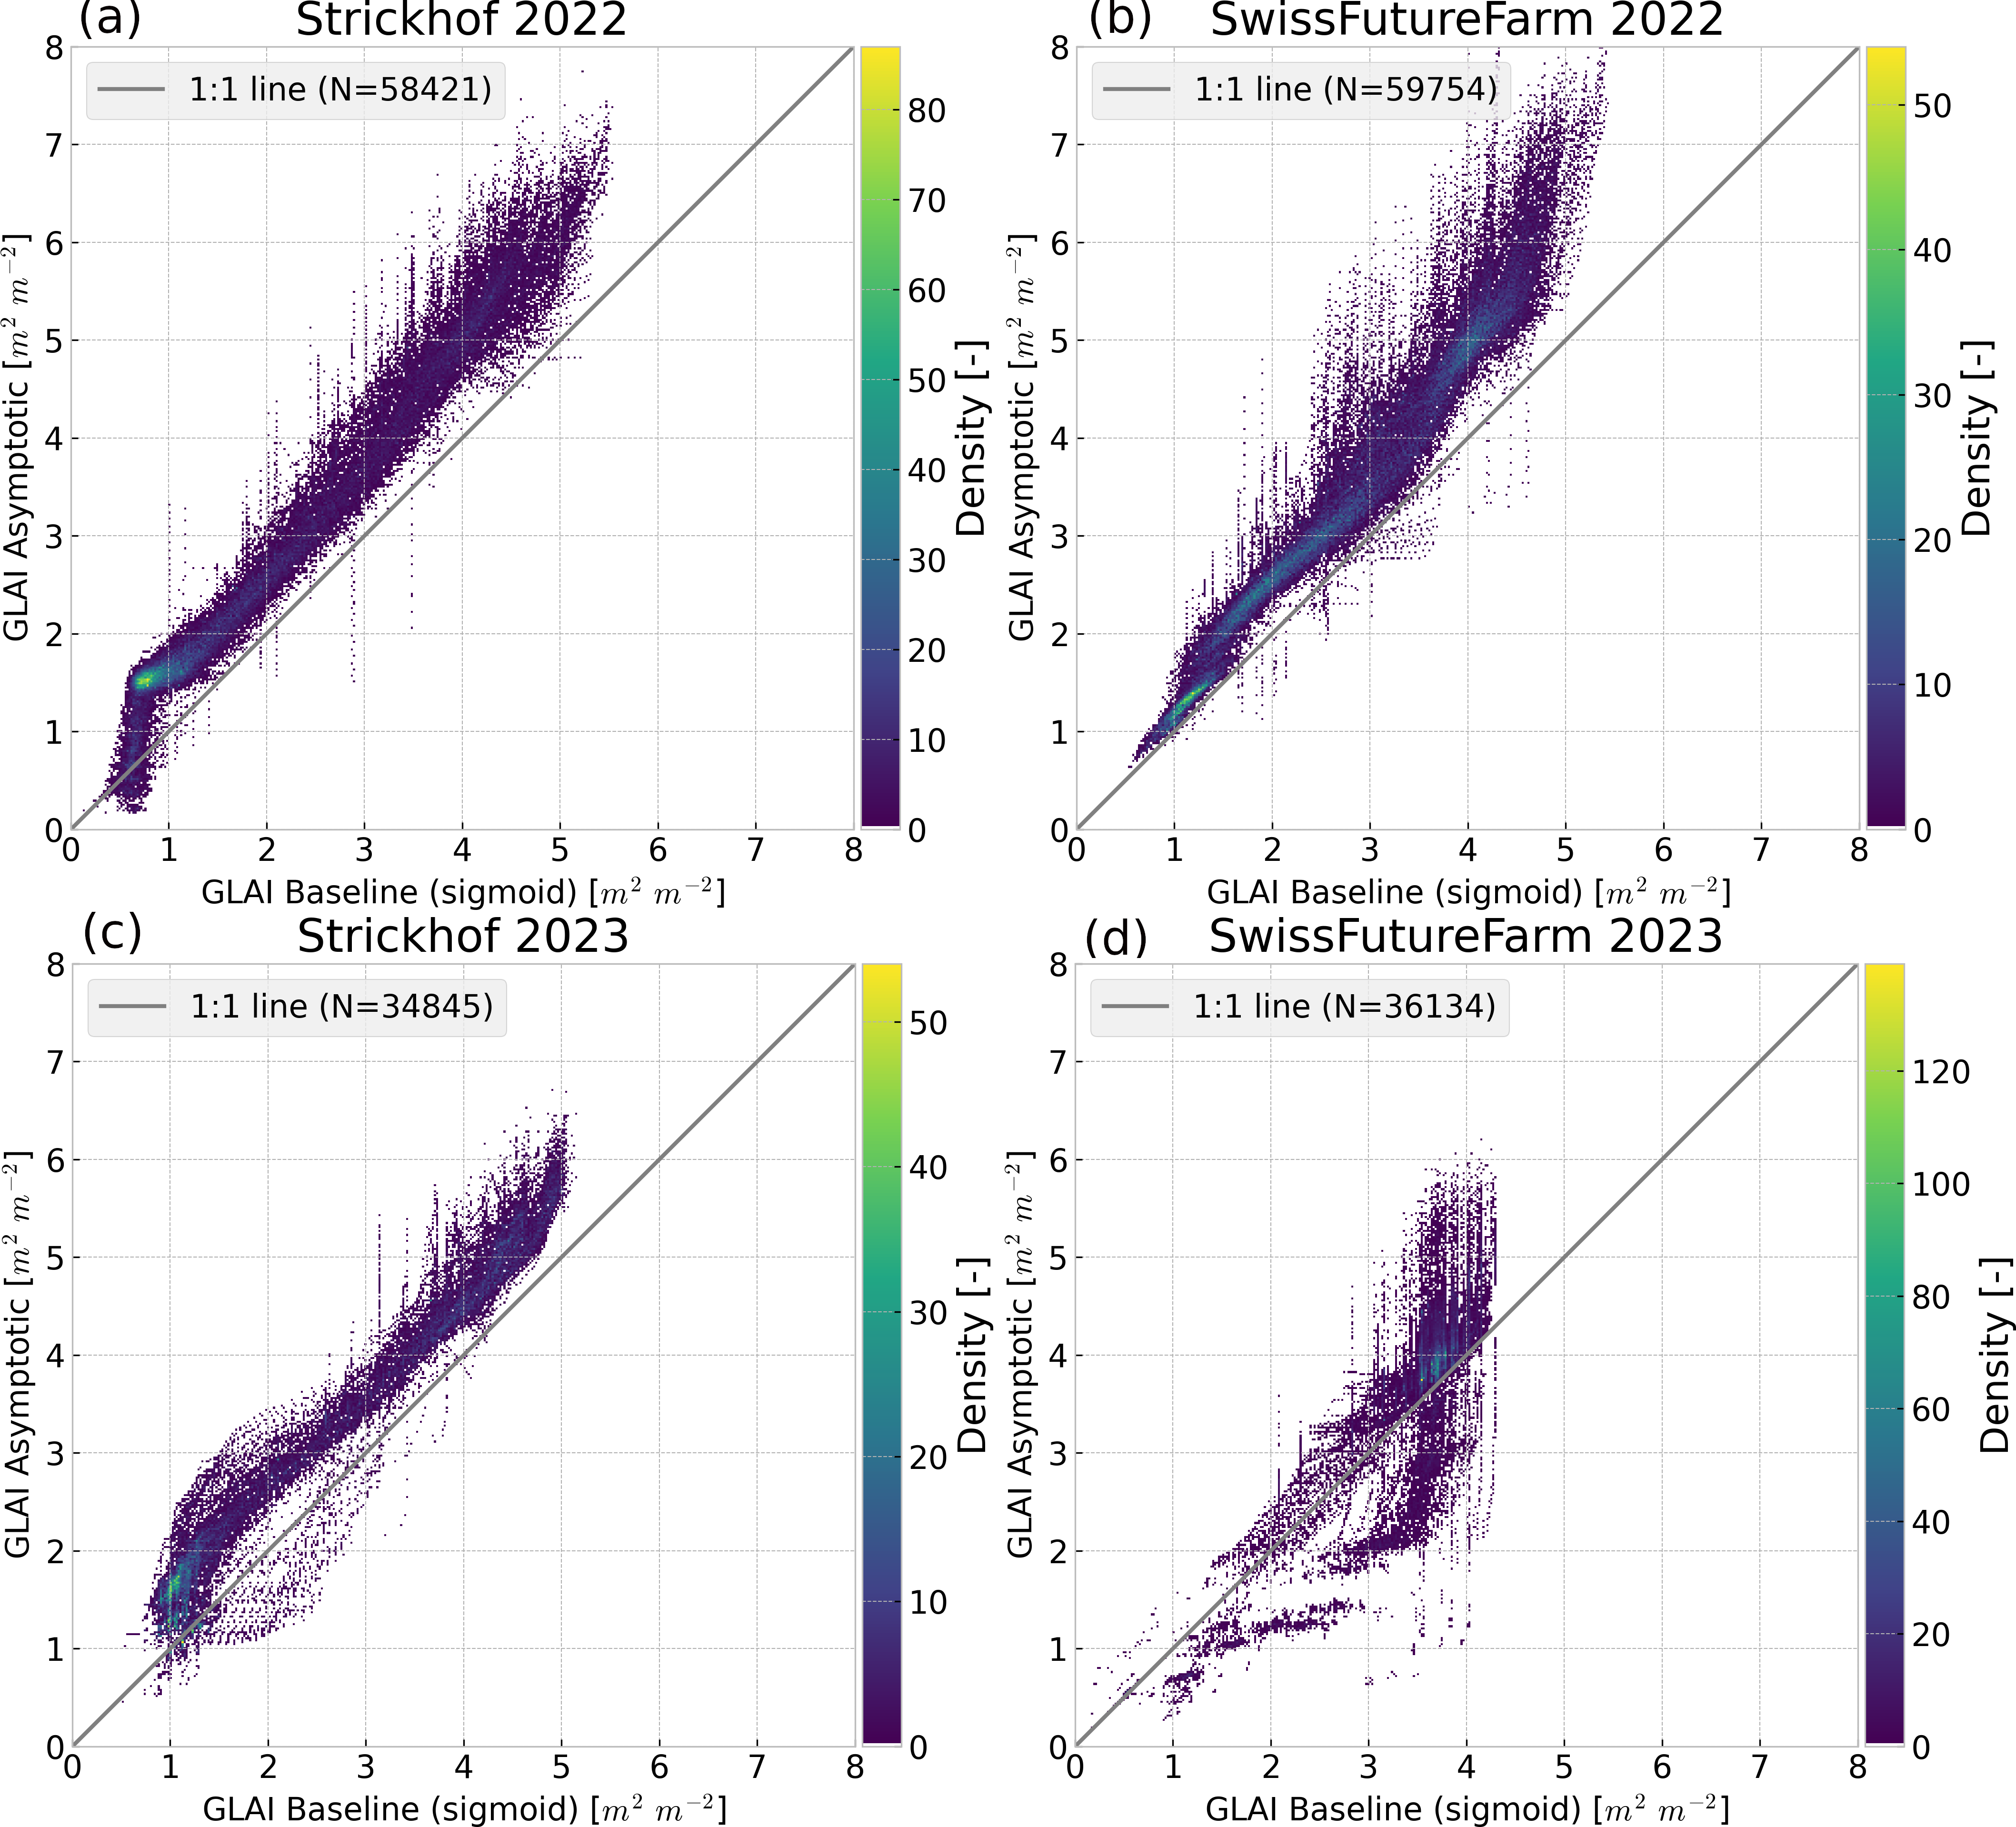
\includegraphics[width=\textwidth]{model_intercomparison_2022-2023.png}
    \caption{Intercomparison of reconstructed GLAI time series values at the Strickhof and Swiss Future Farm sites in 2022 (a, b), and 2023 (c, d), respectively, showing all reconstructed GLAI values from the asymptotic DRC GLAI plotted against all reconstructed baseline GLAI values.}
    \label{fig:model-intercomparison}
\end{figure}


\subsection{GLAI reconstruction success rate}
\label{subsec:glai-reconstruction-sucess}
As described in Section~\ref{subsubsec:baseline-method}, the baseline requires at least four valid raw \gls{S2} \gls{GLAI} values to estimate the function parameters. However, this requirement was not met for all \gls{S2} pixels: While the overall number of \gls{S2} observations is higher than four at all sites (see Section \ref{subsec:s2-imagery}), the \gls{SCL} and simple outlier filtering (Section~\ref{subsubsec:s2-glai-simple-outlier-filter}) caused the total number of valid raw \gls{GLAI} observations to drop below the threshold of four in some cases. Overall, the baseline \gls{GLAI} could not be fitted to 12.43\% of the pixels at the validation sites, with variations from 5.46\% at the Swiss Future Farm in 2022 to 20.08\% at the same site in 2023. The latter case is displayed in Figure \ref{fig:maps-baseline-failure} comparing the daily asymptotic \gls{DRC} \gls{GLAI} to baseline \gls{GLAI} for two dates during late stem elongation and heading. The failure of the baseline to reconstruct \gls{GLAI} values was caused in two thirds of the pixels by a too low number of valid raw \gls{GLAI} observations (< 4), and in one third by the non-convergence of the optimization algorithm after reaching the maximum number of iterations (1000). Although often only pixels at the parcel boundaries were affected, about 40\% of the pixels were located within the parcels, resulting in undesired spatial gaps in the reconstructed baseline \gls{GLAI} (c.f., Figure \ref{fig:maps-baseline-failure}, right). In contrast, for the \gls{DRC} \gls{GLAI}, which only require a minimum number of two valid \gls{GLAI} observations, reconstruction could be performed for all \gls{S2} pixels.

\begin{figure}[H]
    \centering
    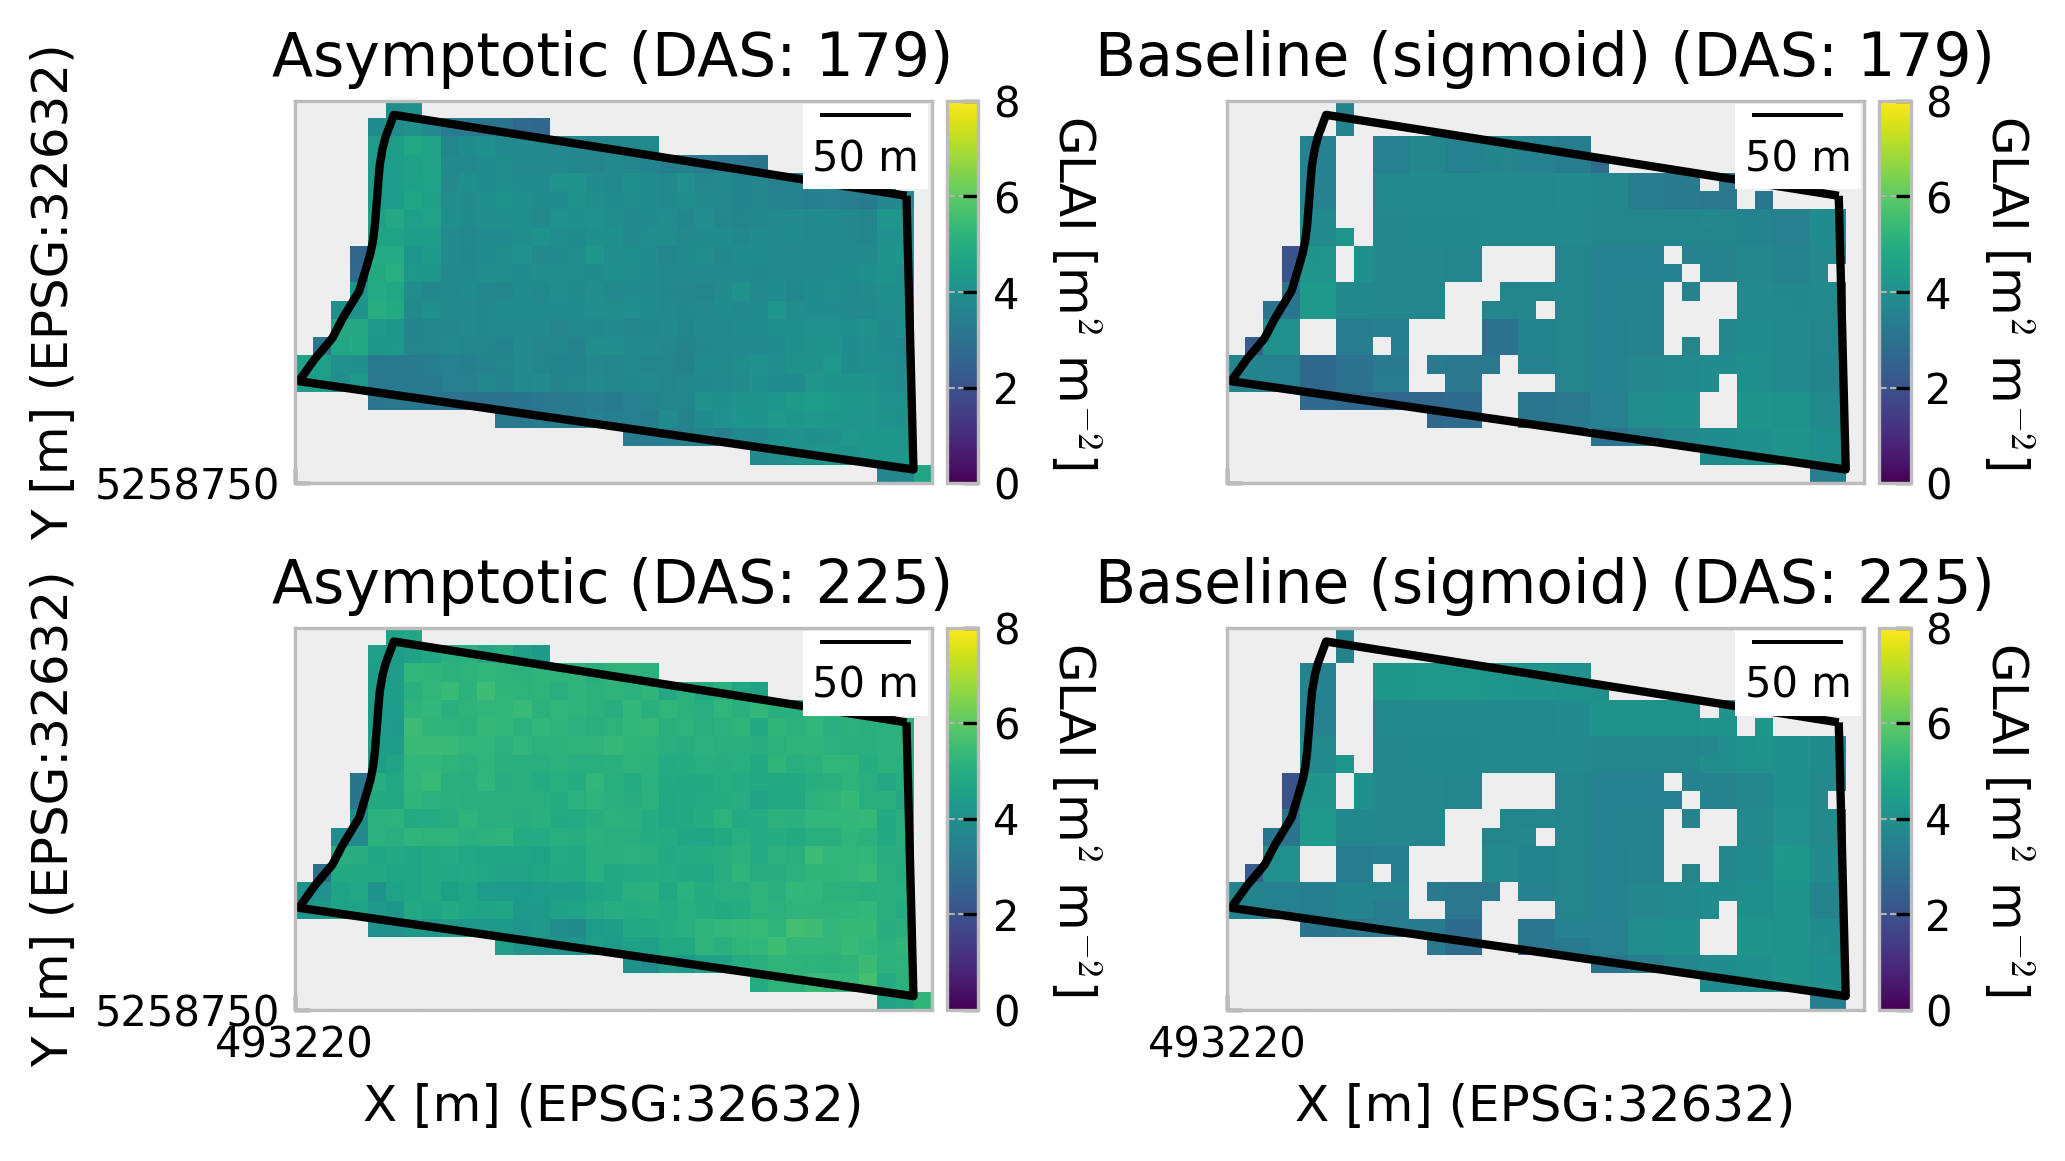
\includegraphics[width=\textwidth]{SwissFutureFarm_2023_Grund_asymptotic-sigmoid.png}
    \caption{Maps of daily asymptotic DRC (left) and baseline GLAI (right) for the parcel Grund at Swiss Future Farm in 2023 for two dates during late stem elongation (top) and heading (bottom) expressed as days after sowing (DAS). The parcel boundary is shown as black line.}
    \label{fig:maps-baseline-failure}
\end{figure}